\section{Introduction To Data Management and Data Warehouse}

%%%%%%%%%%%%%%%%%%%%%%%%%%%%%%%%%%%%%%%%%%%%%%%%%%%%%%%%%%%%%%%%%%%%%%%%%%%%%%%%%%%%%%%%%

\begin{frame}
\frametitle{Chapter Objectives}

\begin{itemize}
	\item<1-> Be familiar with data management life-cycle. \pause
	\item<2-> Introduction to data warehouse and its usage. \pause	
	\item<3-> Motivation to DWH.\pause
	\item<4-> What is the different types of DWH?\pause
	\item<5-> Use cases\pause
	\item<6-> Data Encoding and Formats\pause	
	\item<6-> Challenges to build a DWH.\pause
\end{itemize}

\end{frame}

%%%%%%%%%%%%%%%%%%%%%%%%%%%%%%%%%%%

\subsection{Data Management}

\begin{frame}
\frametitle{Data Management}

\begin{itemize}
	\item Data are a product.
	\item Data product has a life-cycle as following (simplified): 
	\begin{itemize}
		\item \textbf{Question}, Idea, or service.
		\item \textbf{Identifying} the source of information and the data type ex: (text, images, videos, audio, or sensors).
		\item \textbf{Document} all details regarding the data including quality, security, efficiency, and access (consideration during the cycle).
		\item Delivery automation (Tools and Process) AKA \textbf{DevOps} cycle.
		\item \textbf{Extraction} Process (collection).
		\item \textbf{Transformation} ex: (cleansing, Apply business logic, Organize).
		\item \textbf{Loading} or store the transformed data based on our usage or use case.
		\item Business Intelligence (\textbf{BI}) or data discovery (continues process).
		\item \textbf{Integration} and publishing.
		\item Data retention or \textbf{archiving} process ex: (Hot or Cold storage).
	\end{itemize}
\end{itemize}

\end{frame}

%%%%%%%%%%%%%%%%%%%%%%%%%%%%%%%%%%%%%%%%%%%%%%%%%%%%%%%%%%%%%%%%%%%%%%%%%%%%%%%%%%%%%%%%%

\begin{frame}
\frametitle{Data Management Life-Cycle}
\begin{center}			
			\smartdiagramset{circular distance=3.5cm,
				font=\scriptsize,
%				text width=1cm,
				module minimum width=2cm,
				circular distance =3.4cm,
				module minimum height=.1cm,
				arrow tip=to}
			\smartdiagram[circular diagram]{Archiving,Idea, Identify, Document, 				
				 DevOps,Extraction, Loading, BI, Integration}


\end{center}

\end{frame}

%%%%%%%%%%%%%%%%%%%%%%%%%%%%%%%%%%%%%%%%%%%%%%%%%%%%%%


\subsection{From DWH to Big Data}
\begin{frame}
\frametitle{Motivation to Data Warehouse}
\begin{itemize}[<+->]
	\item Data could be a product for some companies.
	\item It could be decision support for other products or businesses.
	\item Reporting the results after pass the data life-cycle will be from storage (Database).
	\item There are some challenges facing the people who work on data management backend:
	\begin{itemize}
		\item Performance.
		\item Integration.
		\item Applying analytical functions. %Moving average
	\end{itemize}
	\item Vendors who are working to solve the above challenges creating their own product of DWH and their ultimate work is to optimize the above points.
\end{itemize}
\end{frame}

%%%%%%%%%%%%%%%%%%%%%%%%%%%%%%%%%%%%%%%%%%%%%%%%%%%%%%
\begin{frame}
\frametitle{Motivation to Data Warehouse (DWH)}

\begin{definition}[What is Data Warehousing?] A DWH is defined as a technique for collecting and managing data from varied sources to \textbf{provide meaningful business insights}. It is a blend of technologies and components which aids the strategic use of data.\footnotemark
\end{definition}
\begin{itemize}
	\item The DWH is not a product but an environment.
	\item It is a process of transforming data into information and making it available to users in a \textbf{timely manner} to make a difference.
	\item It is an architectural construct of an information system which provides users with current and historical decision support information which is difficult to access or present in the traditional operational data store.
	\item The DWH is the core of the BI system which is built for data analysis and reporting.
\end{itemize}
\footnotetext{The definition mentioned in this slides copied from  \href{https://www.guru99.com/data-warehousing.html\#2}{guru99.com} }
\end{frame}

%%%%%%%%%%%%%%%%%%%%%%%%%%%%%%%%%%%%%%%%%%%%%%%%%%%%%%
\begin{frame}
\frametitle{Motivation to Data Warehouse}

Data warehouse system is also known by the following names:


\begin{itemize}
\item Decision Support System (DSS).
\item Business Intelligence Solution.
\item Executive Information System.
\item Management Information System.
\item Analytic Application.
\item Data Warehouse.

\end{itemize}

The real concept was given by Inmon Bill. He was considered as a father of the DWH. He had written about a variety of topics for building, usage, and maintenance of the warehouse \& the Corporate Information Factory

\end{frame}

%%%%%%%%%%%%%%%%%%%%%%%%%%%%%%%%%%%%%%%%%%%%%%%%%%%%%%
\begin{frame}
\frametitle{Motivation to Data Warehouse}
Types of Data Warehouse
	\begin{description}
		\item [\textbf{Enterprise Data Warehouse (EDWH)}] It provides decision support service across the enterprise. It offers a unified approach for organizing and representing data (DWH Model). It offers data classifications according to the subject with privileges policy.
		\item [\textbf{Operational Data Store (ODS):}] is a central database that provides an up-to-date (real-time) data from multiple transnational systems for operational reporting into a single DWH.
		
		%% for real time questions and answers. call ODS using intermidiate data store. DWH is day -1 (billing & subscribtions). Oracle (Loading or headache) && CDC capture change interest column not row
		\item [\textbf{Data Mart:}] A data mart is a subset of the data warehouse. It specially designed for a particular line of business, such as sales, finance, sales or finance. In an independent data mart, data can collect directly from sources.
	\end{description}

\end{frame}

%%%%%%%%%%%%%%%%%%%%%%%%%%%%%%%%%%%%%%%%%%%%%%%%%%%%%%

%%%%%%%%%%%%%%%%%%%%%%%%%%%%%%%%%%%%%%%%%%%%%%%%%%%%%%

\begin{frame}
\frametitle{DWH vs ODS vs Data Mart}


\begin{table}[t]
	\centering	
	\resizebox{\columnwidth}{!}{%
		
		%		\centering
		\begin{tabular}{|c | c | c| c |}
			\hline
			\textbf{Metric}  & \textbf{DWH}& \textbf{ODS} & \textbf{Data Mart} \\
			\hline
			Latency & Day -1  & Real-time & Day -1 \\			
			Data level  & Transnational & Transnational & Summary \\
			Historical  & Long-term & Snapshot & Aggregated Long-Term \\
			Size & TB/PB & GB & GB/TB\\
			Orientation & Multi sources & Multi sources & Product\\
			Business Units & Multi organizational units & Product team & Business team \\
			\hline
		\end{tabular}
		%		\caption{Data Representation Combination Matrix}\label{Tab:Data_Representation_Matrix}
	}
\end{table}
\end{frame}


%%%%%%%%%%%%%%%%%%%%%%%%%%%%%%%%%%%%%%%%%%%%%%%%%%%%%%

\begin{frame}
\frametitle{DWH vs Operational databases}
\begin{itemize}[<+->]
		\item Operational databases (Transactions DB) still working as the backend for the products.
		\item Data warehouse mainly works as centralized storage for all the source systems regardless of the product type or their functionality.
		\item Data warehouse designed to solve the \textbf{huge amount of data}.
		\item Most of DWH can't solve the online transactions similar to the transaction DB.
		\item Transactions databases have a performance issue while handling a huge amount of data. So, analysis of a huge amount of data (including historical data) we used DWH for this purpose. On the other hand Transactions DB used for online or short historical data based on product type and requirements.
\end{itemize}
\end{frame}


%%%%%%%%%%%%%%%%%%%%%%%%%%%%%%%%%%%%%%%%%%%%%%%%%%%%%%

\begin{frame}
\frametitle{DWH vs Operational databases}


\begin{table}[t]
\centering	
\resizebox{\columnwidth}{!}{%

%		\centering
		\begin{tabular}{|c | c | c|}
			\hline
			\textbf{Metric}  & \textbf{Transactions DB}& \textbf{DWH} \\
			\hline
			Volume & GB/TB & TB/PB \\
			Historical  & Short-term & Long-Term\\
			rows & <1000M &  1000M>\\
			Orientation & Product & Subject or multi products\\
			Business Units & Product team & Multi organizational units\\
			Normalization & Normalized %due to storage and performance limitation and its design
			 &  Not required (De-normalized in many use cases)\\
			 Data Model & Relational & Star Schema or Multi-dim\\
			 Intelligence&Reporting & Advanced reporting and Machine Learning\\
			 Use cases& Online transactions \& operations & Centeralized storage (360\textdegree)\\
			\hline
		\end{tabular}
%		\caption{Data Representation Combination Matrix}\label{Tab:Data_Representation_Matrix}
}
\end{table}
\end{frame}


%%%%%%%%%%%%%%%%%%%%%%%%%%%%%%%%%%%%%%%%%%%%%%%%%%%%%%

\begin{frame}
\frametitle{Transnational DB Use cases}
\begin{figure}[ht]

		\centering
		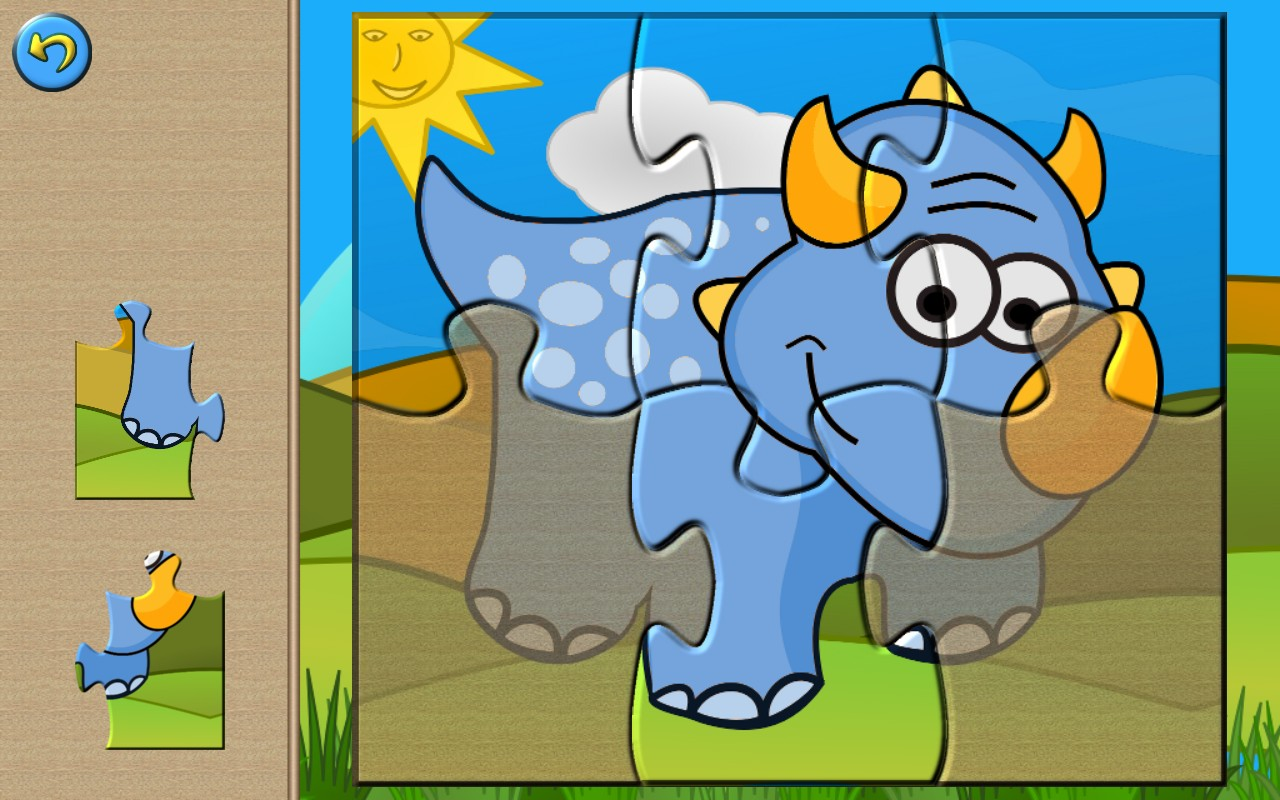
\includegraphics[width=\linewidth]{./Figures/chapter-01/baby-01.jpg}
%		
\includegraphics[width=\linewidth,height=\textheight]{./Figures/chapter-01/baby-02.jpg}
	%	\caption{}
\end{figure}
\end{frame}


%%%%%%%%%%%%%%%%%%%%%%%%%%%%%%%%%%%%%%%%%%%%%%%%%%%%%%
\begin{frame}
\frametitle{Transnational DB Use cases}
\begin{figure}[ht]
	
	\centering
%	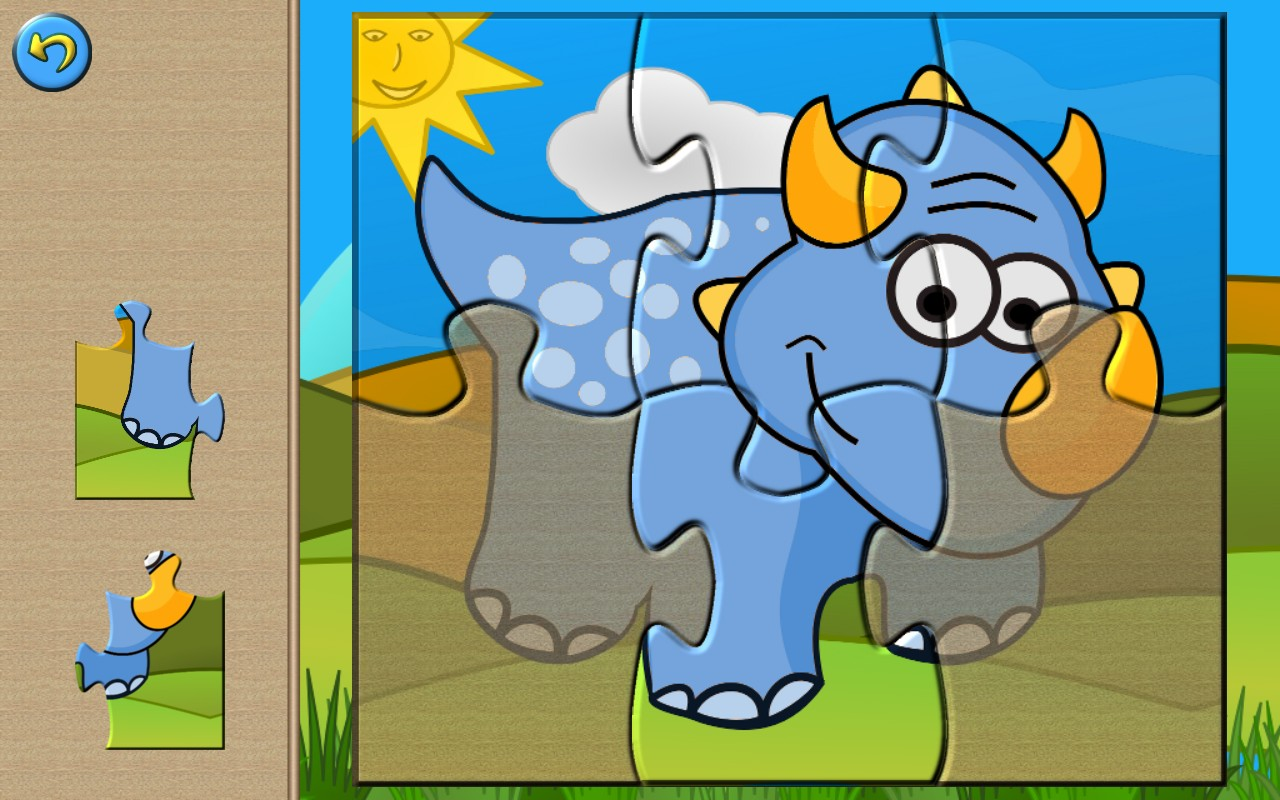
\includegraphics[width=\linewidth]{./Figures/chapter-01/baby-01.jpg}
			
\includegraphics[width=\linewidth]{./Figures/chapter-01/baby-02.jpg}
	%	\caption{}
\end{figure}
\end{frame}


%%%%%%%%%%%%%%%%%%%%%%%%%%%%%%%%%%%%%%%%%%%%%%%%%%%%%%
\begin{frame}
\frametitle{DWH Use cases}
\begin{figure}[ht]
	
	\centering
	
\includegraphics[width=\linewidth,height=.8\textheight]{./Figures/chapter-01/Marvel-03.jpg}
	%	\caption{}
\end{figure}
\end{frame}

%%%%%%%%%%%%%%%%%%%%%%%%%%%%%%%%%%%%%%%%%%%%%%%%%%%%%%
\begin{frame}
\frametitle{DWH Use cases}
\begin{figure}[ht]
	
	\centering
	
\includegraphics[width=\linewidth,height=.8\textheight]{./Figures/chapter-01/Marvel-02.jpg}
	%	\caption{}
\end{figure}
\end{frame}

%%%%%%%%%%%%%%%%%%%%%%%%%%%%%%%%%%%%%%%%%%%%%%%%%%%%%%
\begin{frame}
\frametitle{DWH Use cases}
\begin{figure}[ht]
	
	\centering
	
\includegraphics[width=\linewidth,height=.8\textheight]{./Figures/chapter-01/Marvel-01.jpg}
	%	\caption{}
\end{figure}
\end{frame}
%%%%%%%%%%%%%%%%%%%%%%%%%%%%%%%%%%%%%%%%%%%%%%%%%%%%%%

User stories Telecom company.

It has a CRM System backend database reporting the sales. vs Another backend database contains the CRM, Telecom signaling data, IN charging system, Billing

Decision is related to sales or CRM. Decision is related to company strategies.
Analytical model checking the fraud which require a CRM data with customer locations from signaling with Billing details from CAR table.
%%%%%%%%%%%%%%%%%%%%%%%%%%%%%%%%%%%%%%%%%%%%%%%%%%%%%%


%%%%%%%%%%%%%%%%%%%%%%%%%%%%%%%%%%%%%%%%%%%%%%%%%%%%%%
managing risk of the project in Transaction vs DWH


%%%%%%%%%%%%%%%%%%%%%%%%%%%%%%%%%%%%%%%%%%%%%%%%%%%%%%


%%%%%%%%%%%%%%%%%%%%%%%%%%%%%%%%%%%%%%%%%%%%%%%%%%%%%%
data model comparison


%%%%%%%%%%%%%%%%%%%%%%%%%%%%%%%%%%%%%%%%%%%%%%%%%%%%%%

\begin{frame}
\frametitle{DWH Characteristics}

some details about hot vs cold storage,

\end{frame}

%%%%%%%%%%%%%%%%%%%%%%%%%%%%%%%%%%%%%%%%%%%%%%%%%%%%%%


\begin{frame}

\frametitle{Cold storage vs Hot storage}

some details about hot vs cold storage,

\end{frame}


%%%%%%%%%%%%%%%%%%%%%%%%%%%%%%%%%%%%%%%%%%%%%%%%%%%%%%

\subsection{Data Encoding and Formats}
\begin{frame}
\frametitle{\subsecname}
\begin{itemize}[<+->]
	\item Any Big Data solution working based distributed systems.
	\item What is distributed systems in brief?
\end{itemize}
\end{frame}

%%%%%%%%%%%%%%%%%%%%%%%%%%%%%%%%%%%%%%%%%%%%%%%%%%%%%%

\subsection{Assignment and Homework}


%%%%%%%%%%%%%%%%%%%%%%%%%%%%%%%%%%%%%%%%%%%%%%%%%%%%%%%%%%%%%%%%%%%%%%%%%%%
%%% Local Variables:
%%% mode: latex
%%% TeX-master: "../main"
%%% TeX-engine: xetex
%%% End:
